\captionsetup{justification=centering,margin=0cm}
\label{cap:atividade1}  % Forma de referenciar o capítulo no comando \ref

%inicio do capitulo
\chapter[Atividade 1: Investigando formatos e características de arquivos de vídeo.]{Atividade 1: Investigando formatos e características de arquivos de vídeo.}

Nesta atividade iremos observar alguns dados técnicos de maneira breve os \textit{containers}, avaliando principalmente o elemento vídeo.

\section{Atividade 1A - Investigando os arquivos de vídeo fornecidos}

\begin{figure}[H]
    \centering
    \caption{Informações do primeiro \textit{container} avaliado}
    \label{fig:imagem1}
    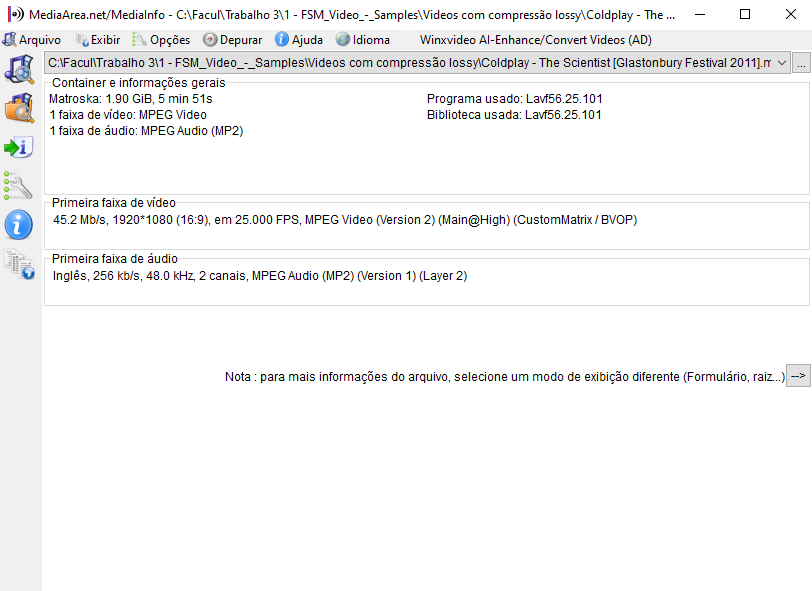
\includegraphics[scale=0.5]{Documeto/1-ElementosTextuais/images/01.png}
    
    \autoriaPropria
\end{figure}

Observo que neste \textit{container} tem um tamanho total do arquivo 1.90 GigaByte, um video de 5 minutos de 51 segundos no formato MPEG e apenas uma faixa de áudio (mono) MPEG Audio (MP2). Trata-se de um vídeo com amostragem espacial em FHD, que tem 1920 colunas por 1080 linhas progressivas em uma proporção 16x9 (a cada 16 colunas existem 9 linhas e vice-versa).

\paragrafo O aplicativo também revela que o \textit{Frame Rate} (FPS) está em 25 (amostragem temporal muito próxima às dos cinemas tradicionais) , onde para cada segundo são necessários em média 45,2 Mb de armazenamento, e a língua nativa do áudio (inglesa).
O programa/biblioteca utilizado irei relevar pois não os conheço. Este vídeo é evidentemente extremamente mal otimizado e inutilizável para uso online.

\begin{figure}[H]
    \centering
    \caption{Informações do primeiro \textit{container} avaliado}
    \label{fig:imagem2}
    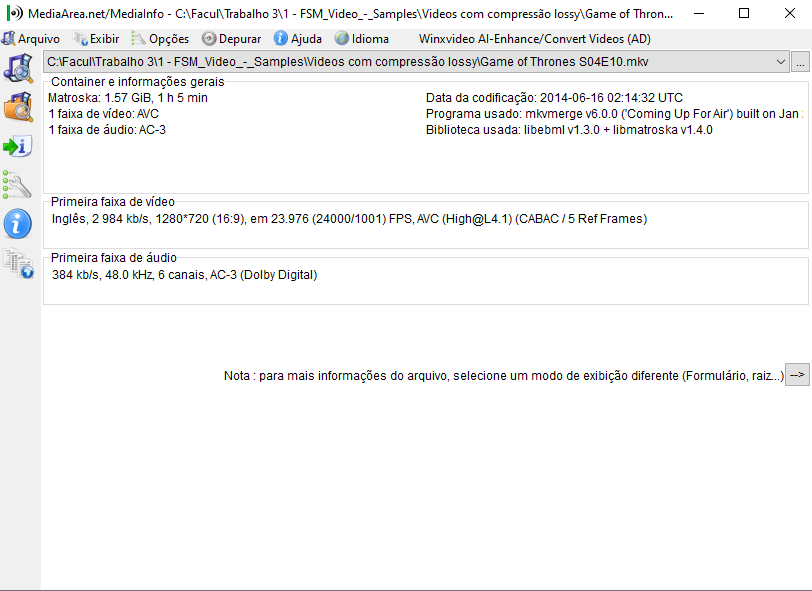
\includegraphics[scale=0.5]{Documeto/1-ElementosTextuais/images/02.png}
    
    \autoriaPropria
\end{figure}

\paragrafo Observo que neste container tem um tamanho total do arquivo 1.90 GigaByte, um video de 5 minutos de 51 segundos no formato MPEG e apenas uma faixa de audio (mono) MPEG Audio (MP2). Trata-se de um vídeo com amostragem espacial em FHD, que tem 1920 colunas por 1080 linhas progressivas em uma proporção 16x9 (a cada 16 colunas existem 9 linhas e vice-versa).

\paragrafo O aplicativo também revela que o Frame Rate (FPS) está em 25 (Amostragem temporal muito próxima às dos cinemas tradicionais) , onde para cada segundo são necessários em média 45,2 Mb de armazenamento, e a língua nativa do áudio (inglesa). O programa/biblioteca utilizado irei relevar pois não os conheço. Este vídeo é evidentemente extremamente mal otimizado e inutilizável para uso online. Este vídeo já pesaria para rodar online. Outro vídeo extremamente pesado.

\begin{figure}[H]
    \centering
    \caption{Informações do primeiro \textit{container} avaliado}
    \label{fig:imagem3}
    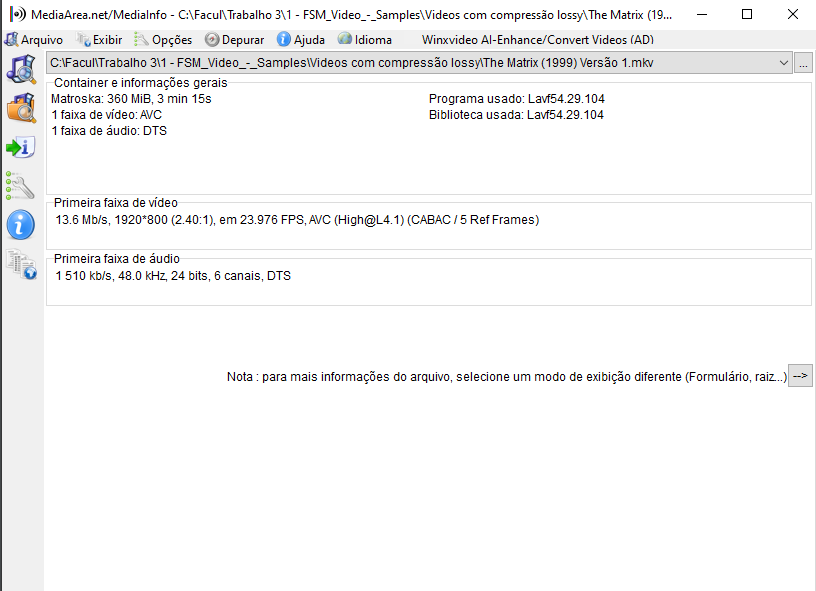
\includegraphics[scale=0.5]{Documeto/1-ElementosTextuais/images/03.png}
    
    \autoriaPropria
\end{figure}

\begin{figure}[H]
    \centering
    \caption{Informações do primeiro \textit{container} avaliado}
    \label{fig:imagem4}
    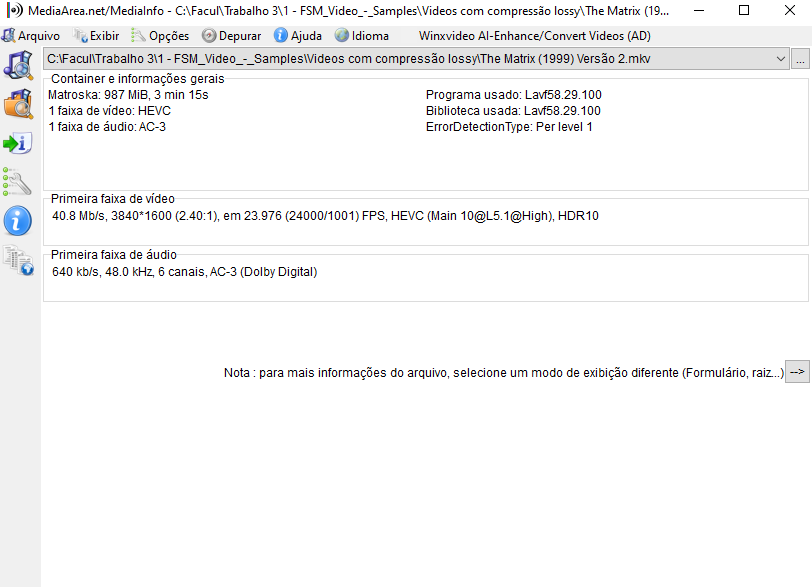
\includegraphics[scale=0.5]{Documeto/1-ElementosTextuais/images/04.png}
    
    \autoriaPropria
\end{figure}


\section{Atividade 1B - Investigando vídeos originados de HDTV Europeu}

Sendo esses detalhes mais relevantes para aquele que vai disponibilizar para visualização, mas agora passar a ver do lado de quem vai ver o vídeo, analisando o vídeo de Coldplay - The Scientist do Festival Glastonbury de 2011 (Uma música MUITO boa por sinal).
\paragrafo Assistindo ao vídeo, nota-se que tem uma qualidade muito boa (No mínimo né, já que é um arquivo de quase 2 gigas para menos de 6 minutos) em um player de vídeo, entretanto ao utilizar o Avidemux, podemos analisar o vídeo frame a frame.
\paragrafo Ao analisar os pontos de maior probabilidade de artefatos, temos os locais com grande movimentação, muitos tons escuros diferentes, pequenos objetos se movimentando e alto contraste.
Ao observar o video mais calmamente, obtemos uma imagem como a demonstrada nas imagens abaixo:

\begin{figure}[H]
    \centering
    \caption{Informações do primeiro \textit{container} avaliado}
    \label{fig:imagem5}
    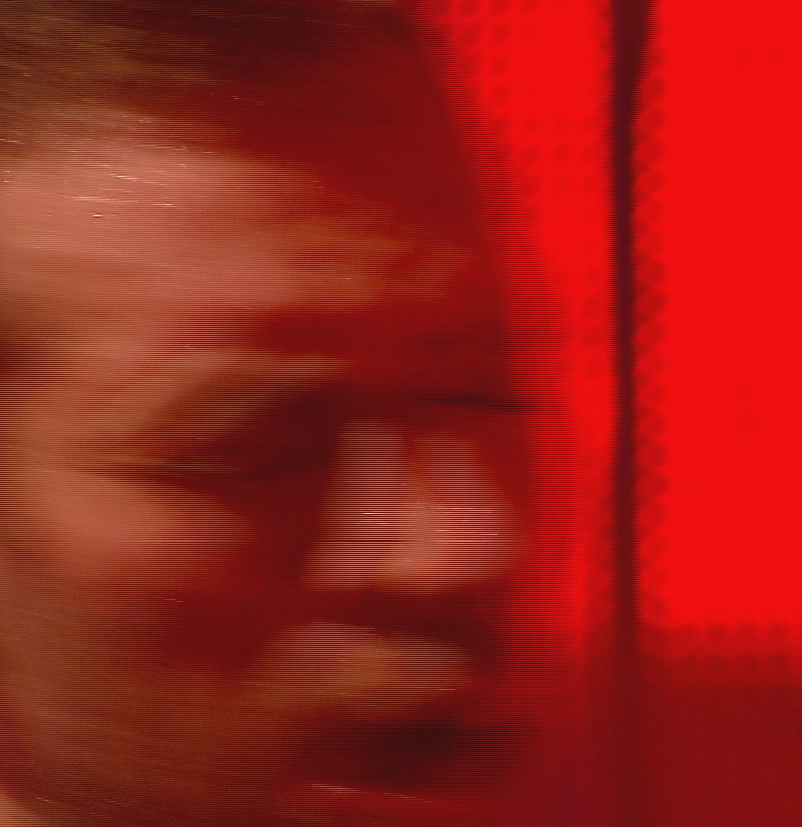
\includegraphics[scale=0.5]{Documeto/1-ElementosTextuais/images/05.png}
    
    \autoriaPropria
\end{figure}

Nestes casos, o artefato ocorreu por uma grande movimentação do cantor em um curto intervalo de tempo, fazendo a tela ficar toda borrada nesta amostra espacial. E aqui ruído de mosquito nos instrumentos pelo alto contraste.

\begin{figure}[H]
    \centering
    \caption{Informações do primeiro \textit{container} avaliado}
    \label{fig:imagem6}
    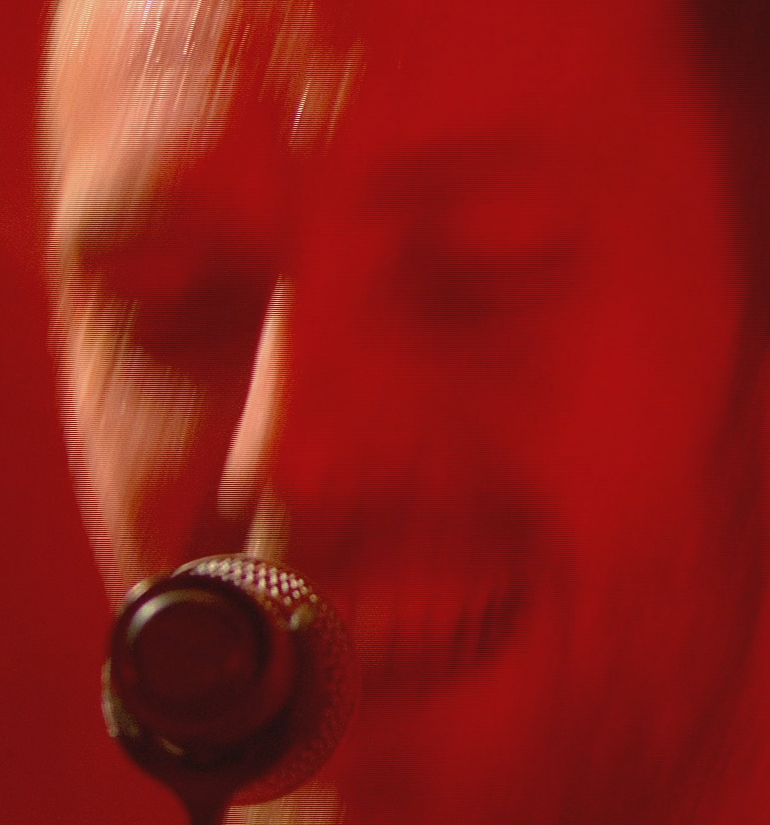
\includegraphics[scale=0.5]{Documeto/1-ElementosTextuais/images/06.png}
    
    \autoriaPropria
\end{figure}

\paragrafo Mas apesar de ser bem visível ao passar frame a frame, é imperceptível ao olhar-los em sequência a 25 FPS como o vídeo foi configurado para ser reproduzido, isso se deve a uma característica humana, em que não somos capazes de analisar as imagens separadamente, então o cérebro une as imagens e cria uma sensação de movimento, além inventar informação para partes que não está em foco. Resultando em um vídeo fluido e com boa qualidade (é muito estranho ver uma fumaça tão bem representada quanto nesse clipe).

\begin{figure}[H]
    \centering
    \caption{Informações do primeiro \textit{container} avaliado}
    \label{fig:imagem7}
    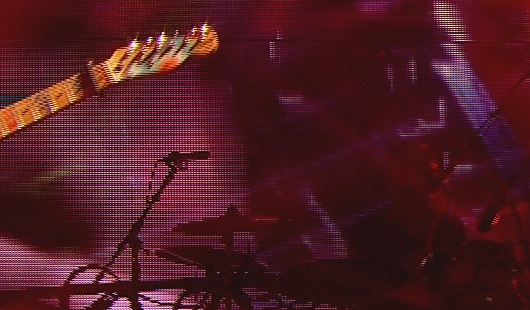
\includegraphics[scale=0.5]{Documeto/1-ElementosTextuais/images/07.png}
    
    \autoriaPropria
\end{figure}

\paragrafo No entanto, também há um detalhe que torna esse vídeo inviável de ser transmitido, seu tamanho. Após breve pesquisa no suporte do google \url{https://support.google.com/youtube/answer/78358?hl=pt-BR}, é evidente que um fluxo de dados recomendados para vídeos em FHD é de 5Mbps, o que está longe de ser a realidade do vídeo analisado (sendo ele 45,2 Mbps), está MUITO acima do recomendado e não sendo apropriado para streaming online.


\section{Atividade 1C - Investigando os formatos usados pelo Youtube}
Agora partiremos para uma análise do que é apropriado para um site de streaming, iremos observar os diferentes CODECs e a eficiência delas para vídeo.
Na tabela abaixo estão todos os formatos de vídeo capturados pelo Jdownloader 2 do vídeo “Best of 8K HDR 60p (FUHD)” no youtube.

\begin{table}[H]
    \centering
    \caption{Tabela 1}
    \label{tab:tabela1}
    \begin{tabularx}{\textwidth}{X|C|C|C|C|C}
        \hline
         \textbf{Resolução} & \textbf{Frame Rate} & \textbf{Codec} & \textbf{Formato do Contêiner} & \textbf{Bitrate Geral (kb/s)} & \textbf{Tamanho (MiB)} \\ \hline
        144 & 30 & VP9 & MKV & 200 & 6,2 \\ \hline
        144 HDR & 60 & VP9 & MKV & 321 & 9,94 \\ \hline
        240 & 30 & VP9 & MKV & 265 & 8,23 \\ \hline
        240 HDR & 60 & VP9 & MKV & 547 & 17 \\ \hline
        360 & 30 & VP9 & MKV & 461 & 14,3 \\ \hline
        360 HDR & 60 & VP9 & MKV & 1057 & 32,8 \\ \hline
        480 & 30 & VP9 & MKV & 603 & 18,7 \\ \hline
        480 HDR & 60 & VP9 & MKV & 1973 & 61,1 \\ \hline
        720 & 30 & VP9 & MKV & 1132 & 35,1 \\ \hline
        720 HDR & 60 & VP9 & MKV & 4440 & 138 \\ \hline
        720 & 60 & VP9 & MKV & 2232 & 69,2 \\ \hline
        1080 HDR & 60 & VP9 & MKV & 6725 & 208 \\ \hline
        1080 & 60 & VP9 & MKV & 3591 & 111 \\ \hline
        1440 HDR & 60 & VP9 & MKV & 16200 & 502 \\ \hline
        1440 & 60 & VP9 & MKV & 10300 & 320 \\ \hline
        2160 HDR & 60 & VP9 & MKV & 28800 & 894 \\ \hline
        2160 & 60 & VP9 & MKV & 23900 & 739 \\ \hline
        144 & 30 & H-264/AVC & MP4 & 187 & 5,79 \\ \hline
        144s & 60 & AV1 & MP4 & 257 & 7,97 \\ \hline
        240 & 30 & H-264/AVC & MP4 & 262 & 8,13 \\ \hline
        240 & 60 & AV1 & MP4 & 398 & 12,3 \\ \hline
        360 & 30 & H-264/AVC & MP4 & 414 & 12,8 \\ \hline
        360 & 60 & AV1 & MP4 & 690 & 21,4 \\ \hline
        480 & 30 & H-264/AVC & MP4 & 614 & 19 \\ \hline
        480 & 60 & AV1 & MP4 & 1199 & 37,2 \\ \hline
        720 & 30 & H-264/AVC & MP4 & 1670 & 51,7 \\ \hline
        720 & 60 & AV1 & MP4 & 3.170 & 98,3 \\ \hline
        720 & 60 & H-264/AVC & MP4 & 2.752 & 85,3 \\ \hline
        1080 & 60 & AV1 & MP4 & 5.010 & 155 \\ \hline
        1080 & 60 & H-264/AVC & MP4 & 4.838 & 150 \\ \hline
        1440 & 60 & AV1 & MP4 & 13900 & 431 \\ \hline
        2160 & 60 & AV1 & MP4 & 24600 & 763 \\ \hline
        144 & 30 & VP9 & WEBM & 128 & 3,97 \\ \hline
        144 & 30 & VP9 & WEBM & 176 & 5,47 \\ \hline
        144 HDR & 60 & VP9 & WEBM & 249 & 7,71 \\ \hline
        144 HDR & 60 & VP9 & WEBM & 297 & 9,21 \\ \hline
        240 & 30 & VP9 & WEBM & 193 & 6 \\ \hline
        240 & 30 & VP9 & WEBM & 242 & 7,5 \\ \hline
        240 HDR & 60 & VP9 & WEBM & 475 & 14,7 \\ \hline
        240 HDR & 60 & VP9 & WEBM & 524 & 16,2 \\ \hline
    \end{tabularx}

    \autoriaPropria
\end{table}

\begin{table}[H]
    \centering
    \caption{Tabela 1 - Continuação}
    \label{tab:tabela1-continuacao}
    \begin{tabularx}{\textwidth}{X|C|C|C|C|C}
        \hline
         \textbf{Resolução} & \textbf{Frame Rate} & \textbf{Codec} & \textbf{Formato do Contêiner} & \textbf{Bitrate Geral (kb/s)} & \textbf{Tamanho (MiB)} \\ \hline
        360 & 30 & VP9 & WEBM & 389 & 12,1 \\ \hline
        360 & 30 & VP9 & WEBM & 438 & 13,6 \\ \hline
        360 HDR & 60 & VP9 & WEBM & 985 & 30,5 \\ \hline
        360 HDR & 60 & VP9 & WEBM & 1033 & 32 \\ \hline
        480 & 30 & VP9 & WEBM & 531 & 16,5 \\ \hline
        480 & 30 & VP9 & WEBM & 580 & 18 \\ \hline
        480 HDR & 60 & VP9 & WEBM & 1901 & 58,9 \\ \hline
        480 HDR & 60 & VP9 & WEBM & 1949 & 60,4 \\ \hline
        720 & 30 & VP9 & WEBM & 1060 & 32,9 \\ \hline
        720 & 30 & VP9 & WEBM & 1109 & 34,4 \\ \hline
        720 HDR & 60 & VP9 & WEBM & 4368 & 135 \\ \hline
        720 HDR & 60 & VP9 & WEBM & 4417 & 137 \\ \hline
        720 & 60 & VP9 & WEBM & 2160 & 67 \\ \hline
        720 & 60 & VP9 & WEBM & 2209 & 68,5 \\ \hline
        1080 HDR & 60 & VP9 & WEBM & 6654 & 206 \\ \hline
        1080 HDR & 60 & VP9 & WEBM & 6702 & 208 \\ \hline
        1080 & 60 & VP9 & WEBM & 3519 & 109 \\ \hline
        1080 & 60 & VP9 & WEBM & 3568 & 111 \\ \hline
        1440 HDR & 60 & VP9 & WEBM & 16100 & 499 \\ \hline
        1440 HDR & 60 & VP9 & WEBM & 16200 & 501 \\ \hline
        1440 & 60 & VP9 & WEBM & 10300 & 318 \\ \hline
        1440 & 60 & VP9 & WEBM & 10300 & 319 \\ \hline
        2160 HDR & 60 & VP9 & WEBM & 28800 & 892 \\ \hline
        2160 HDR & 60 & VP9 & WEBM & 28800 & 893 \\ \hline
        2160 & 60 & VP9 & WEBM & 23800 & 737 \\ \hline
        2160 & 60 & VP9 & WEBM & 23800 & 739 \\ \hline
    \end{tabularx}

    \autoriaPropria
\end{table}

 \paragrafo Já de início, percebe-se que dentre os formatos do grupo MPEG, apenas o formato H-264/AVC está presente. Pode-se dizer que o motivo disto, é a rivalidade entre o grupo AV1 (Como o google é um membro fundador, consequentemente, a youtube, vai aderir a rivalidade) e o Grupo MPEG, devido a seu patenteamento descentralizado e caro.

 \paragrafo Dentre os formatos presentes, são apenas 3, VP9, AVC e o AV1. Ao dar foco ao Bitrate dos formatos, nota-se que o formato VP9 no container WEBM é o que mais se destaca, entretanto, há uma grande inconsistência em relação ao HDR - recurso que aumenta utilização (se o hardware tiver compatibilidade) de bits de cor, indo de 24 bits para 30 (10 para cada cor do espectro RBG) - Ele aumentou em grande proporção o tamanho ocupado pelos arquivos pra além do efeito de naturalmente possuir o dobro de quadros, mais que dobrando em resoluções abaixo de 1440p.

\paragrafo Ao comparar os codec, percebemos uma disparidade com a saturação dos vídeos de maneira expressiva na qualidade 1080p. O formato AV1 ficou EXTREMAMENTE ESTOURADO e nos demais foi moderado, onde o melhor deles foi o VP9 sem HDR em nossa opinião. Dessarte, vemos que o formato AV1 não seja tão interessante para monitores e celulares por motivos práticos, provavelmente se adequando a televisão, e o VP9 para o restante e claro, para dispositivos que suportam HDR, vídeos com HDR.

\paragrafo Já analisando apenas o CODEC H.264/AVC em 720p conseguimos observar a diferença de um vídeo a 30 e 60 FPS. E o resultado é grande, vendo primeiro o vídeo em 30 FPS não se vê muita coisa diferente ou de incomum, entretanto comparando as duas qualidades em um curto período de tempo, a diferença é muito perceptível. No movimento do olho do camaleão, dos pássaros voando, no vestido ao vento, em tudo aquilo que possui maior movimentação, tudo é muito mais fluido e temporariamente detalhado, fazendo valer a pena um vídeo maior, como é o caso, para se ter 60 quadros por segundo.

\section{Atividade 1D - Investigando a câmera do seu smartphone e os transcodings feitos pelo Whatsapp e Telegram}
A seguinte atividade visa verificar a influência dos codecs de vídeo dos softwares de mensagem Whatsapp e Telegram. No total, 4 vídeos foram gravados, dois a uma taxa média aproximada de 30 quadros por segundo (FPS) e outros dois a uma taxa média aproximada de 60 quadros por segundo. Todos os quatro vídeos possuem gravações em um mesmo local, ou seja, as informações são semelhantes, no entanto, um par (composto por um vídeo a 30 e outro a 60) foi gravado com maior velocidade de movimento, enquanto o outro com uma menor taxa de movimento.

\paragrafo Cada vídeo foi transferido ao respectivo aplicativo e então comparado com os arquivos originais. Em relação ao Whatsapp, a qualidade fica nitidamente inferior em relação ao original. Há muito ruído em regiões mais escuras; em regiões mais claras também é possível perceber perdas de qualidade, mas não em tanta intensidade. Ademais, textos em particular foram muito prejudicados. Durante o vídeo, há uma carta em papel branco com letras pretas; como já observado em imagem, esse tipo de composição costuma ter bordas bem definidas, o que implica em uma zona de alta complexidade. Esses pontos ficaram tão borrados, que depois de um afastamento de aproximadamente uns 3 metros é preciso fazer um esforço considerável para conseguir compreender as letras. Por fim, a percepção da diferença entre os arquivos de 30 FPS e 60 FPS podiam ser observadas, mas de forma bem menos nítida do que no arquivo original.

\paragrafo Já no Telegram, a situação foi consideravelmente diferente. O encoder da ferramenta deixou o vídeo bem mais polido e com menos perdas grotescas de qualidade. Comparado ao original, os arquivos estão relativamente próximos. A taxa de ruído de mosquito ainda é perceptível na maior parte do tempo, no entanto é bem menor do que no Whatsapp. Além disso, o texto teve um aumento de qualidade considerável, a uma distância semelhante ao software concorrente o texto ainda pode ser lido com facilidade. Por fim, a diferença entre os arquivos em 30FPS e 60FPS é bastante perceptível.

\paragrafo A fim de evitar interpretações demasiadamente baseadas no método empírico, verificamos as informações dos vídeos no software “MediaInfo”. Nele observamos que o Whatsapp e Telegram adotam estratégias diferentes de compressão. Primeiro, ambos converteram o vídeo do formato HEVC para o formato AVC, no entanto, o primeiro utilizou o “Level 3” (parâmetro que indica uma série de informações para o codec), enquanto o segundo utilizou o “Level 1” (não pensamos em uma explicação para tal). No entanto, o mais importante a ser destacado é que a resolução original em 1920*1080 foi reduzida para 848*480 no Whatsapp, fato não observado no Telegram. Isso justifica a baixíssima qualidade do vídeo no software verde.

\paragrafo De forma mais ampla, julgamos acertado a decisão do Telegram nos parâmetros escolhidos para o seu codec. De acordo com os nossos testes, a qualidade da imagem no Telegram é muito superior ao Whatsapp ao custo aproximado do dobro do arquivo. Uma explicação provável é que o  WhatsApp tomou essa decisão para evitar o acúmulo excessivo de informação no dispositivo do usuário, uma vez que os backups são locais e em plataformas como o Google Drive do usuário. Além disso (e também um motivo mais plausível), o Telegram tinha humildes 550 Milhões de usuários mensais ativos, enquanto o Whatsapp 2 bilhões, uma pequenina diferença. Com um tráfego tão grande de informações, vídeos em qualidade muito elevada não são viáveis.
